For the attractive-repulsive interaction potential $K_{\alpha,\beta}(r)$, the full operator is given by
\begin{align*}
  \mathcal{Q}_{\alpha, \beta}[\hat{\rho}](\hatvec{x}) & := \int_{B_R(\vec{0})} K_{\alpha,\beta}\left(\norm{\hatvec{x} - \hatvec{y}}\right) \hat{\rho}(\hatvec{y}) \,\dd\hatvec{y}                                                               \\
                                                      & = \int_{B_R(\vec{0})} \left(\frac{\norm{\hatvec{x} - \hatvec{y}}^\alpha}{\alpha} - \frac{\norm{\hatvec{x} - \hatvec{y}}^\beta}{\beta}\right) \hat{\rho}(\hatvec{y}) \,\dd\hatvec{y}     \\
                                                      & = \int_{B_1(\vec{0})} \left(\frac{R^\alpha \norm{\vec{x} - \vec{y}}^\alpha}{\alpha} - \frac{R^\beta \norm{\vec{x} - \vec{y}}^\beta}{\beta}\right) \hat{\rho}(R\vec{y}) \, R^d\dd\vec{y} \\
                                                      & = R^d\int_{B_1(\vec{0})} \left(\frac{R^\alpha}{\alpha}\norm{\vec{x} - \vec{y}}^\alpha - \frac{R^\beta}{\beta} \norm{\vec{x} - \vec{y}}^\beta\right) \rho(\vec{y}) \,\dd\vec{y}          \\
                                                      & = \frac{R^{\alpha+d}}{\alpha} \mathcal{Q}^\alpha[\rho](\vec{x}) - \frac{R^{\beta+d}}{\beta} \mathcal{Q}^\beta[\rho](\vec{x})\,,
\end{align*}
where one needs to carefully handle the variable transform with $\dd\hatvec{y} = R^d \dd\vec{y}$ in $d$ dimensions whereas the vectors themselves obey $\hatvec{y} = R \vec{y}$ as established previously.
In matrix form that is,
\begin{equation}
  Q_{\alpha, \beta} := \frac{R^{\alpha+d}}{\alpha} Q^\alpha - \frac{R^{\beta+d}}{\beta} Q^\beta\,,
  \label{eq:full-attrep-operator}
\end{equation}
for some interval radius $R \in \R^+$.
The full operator for a set of example parameters is depicted in \Cref{fig:attrep-operator}.

\begin{figure}[H]
  \centering
  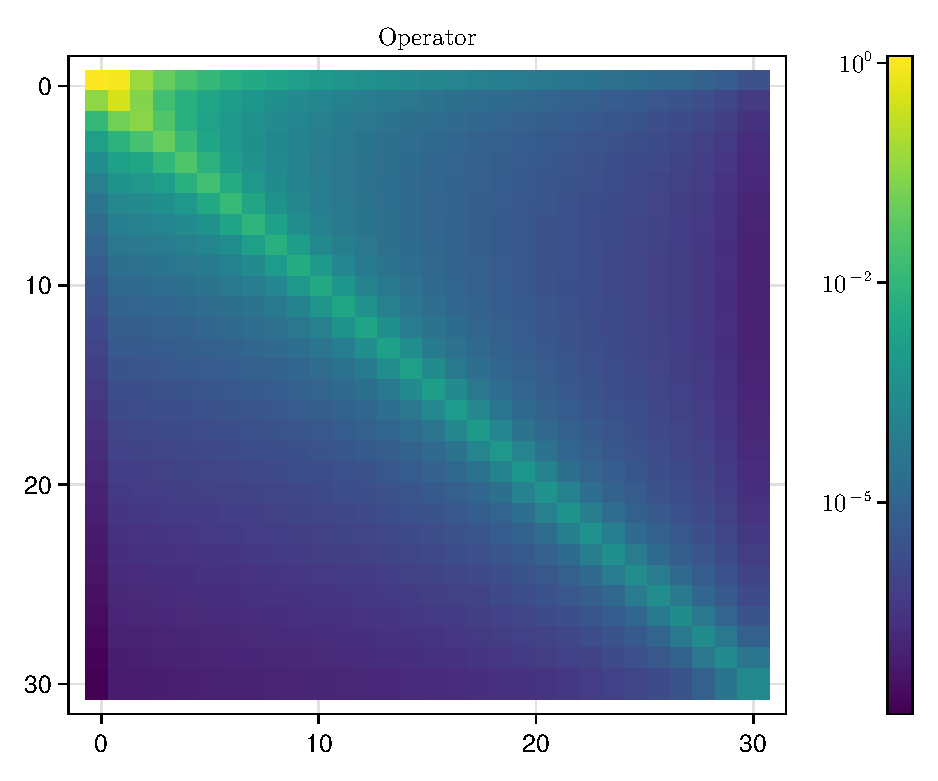
\includegraphics[width=0.5\linewidth]{results/attrep/full-operator.pdf}
  \caption[Combination of the attractive-repulsive operators]{Spy plot of $Q_{\alpha, \beta}$, the combination of the attractive-repulsive operators given in \Cref{fig:attractive-repulsive}. Inverting this operator and applying it to $(1, 0, ..., 0)^T \in \R^N$ will yield the unnormalised coefficients $\rho_k$ of the solution expansion given in \Cref{eq:ansatz}.}
  \label{fig:attrep-operator}
\end{figure}
